\documentclass[11pt]{article}
\usepackage[utf8]{inputenc} % Para caracteres en espa�ol
\usepackage{amsmath,amsthm,amsfonts,amssymb,amscd}
\usepackage{multirow,booktabs}
\usepackage[table]{xcolor}
\usepackage{fullpage}
\usepackage{lastpage}
\usepackage{enumitem}
\usepackage{multicol}
\usepackage{fancyhdr}
\usepackage{mathrsfs}
\usepackage{pdfpages}
\usepackage{wrapfig}
\usepackage{setspace}
\usepackage{esvect}
\usepackage{calc}
\usepackage{multicol}
\usepackage{cancel}
\usepackage{graphicx}
\graphicspath{ {pictures/} }
\usepackage[retainorgcmds]{IEEEtrantools}
\usepackage[margin=3cm]{geometry}
\usepackage{amsmath}
\newlength{\tabcont}
\setlength{\parindent}{0.0in}
\setlength{\parskip}{0.05in}
\usepackage{empheq}
\usepackage{framed}
\usepackage[most]{tcolorbox}
\usepackage{xcolor}
\colorlet{shadecolor}{orange!15}
\parindent 0in
\parskip 12pt
\geometry{margin=1in, headsep=0.25in}
\theoremstyle{definition}
\newtheorem{defn}{Definition}
\newtheorem{reg}{Rule}
\newtheorem{exer}{Exercise}
% Two more packages that make it easy to show MATLAB code
\usepackage[T1]{fontenc}
\usepackage[framed,numbered]{matlab-prettifier}
\lstset{
	style = Matlab-editor,
	basicstyle=\mlttfamily\small,
}
\newtheorem{note}{Note}
\begin{document}  
\setcounter{section}{0}
\thispagestyle{empty}

\begin{center}
{\LARGE \bf Homework 2 Problem 1}\\
{\large AE370 - Spring 2018 \\ Emilio R. Gordon}
\end{center}
\vspace{20mm}
\textbf{Problem:} The function 
\begin{equation*}
\begin{aligned}
f(x) = 2x^3 + 5.875 x^2 - 8.625 x - 24.75
\end{aligned}
\end{equation*}
\newline
has one root in the interval $1 \leq x \leq 4$. Find it using:
\begin{itemize}
\item Bisection
\item the Newton-Raphson method
\item Secant Method
\end{itemize}
\noindent\rule{16.5cm}{0.4pt}
\newline \newline
\textbf{Solution:} Using the algorithms provided in class and the partial matlab code provided from the assignemnt, the function given above produces a single root shown below. As expected, each method produced like results given the specified tollerance of $1 \times 10^{-6}$
\begin{itemize}
\item Bisection: $\hat{x} = 2.062500$
\item Newton-Raphson: $\hat{x} = 2.062500$
\item Secant method: $\hat{x} = 2.062500$
\end{itemize}
Note: If the tolerance were to be decreased, each method would produce different results depending on how loose the tolerance had become. 
\newpage
\textbf{Bisection Method:}
\newline
\newline
Recall that the basic idea of the bisection method is to bracket the root until the interval size is small enough for us to define the root. The algorithm below does just that by finding the middle point between the lower interval and higher interval. After which, we check to see if the root is above or below that middle point. If it is above, then our lower inteval becomes the mid-point. If it is lower, then our higher interval becomes our midpoint. This is repeated until the difference of our high and low intervals is within tolerance. This is shown in Figure 1 below.
\newline
\begin{figure}[h!]
\begin{lstlisting}
function x = bisection(f, x_low, x_high, x_tol)
% Isolate a root of f(x) using bisection.
while x_high-x_low > x_tol
    c = (x_low+x_high)/2;
    if fn(x_low)*fn(c) > 0
        x_low = c;
    else
        x_high = c;
    end
end
x = c;
end
\end{lstlisting}
\caption{Root Finding via Bisection Method}
\end{figure}
\newpage
\textbf{Newton-Raphson Method:}
\newline
\newline
Recall the basic procedure for the Newton-Raphson method:
\begin{shaded}
\begin{itemize}
\item Start from an initial guess of the root $x_1$
\item For each iteration step, $k = 1,2,3,...$
\begin{itemize}
\item check for convergence : $||f(x_k)|| < Tolerance$
\item if so, exit: you have found the approximate root
\item if not, compute the correction increment : $\Delta x_k = - \frac{f(x_k)}{f'(x_k)}$
\item then update the solution: $x_{k+1} = x_k + \Delta x_k$
\end{itemize}
\end{itemize}
\end{shaded}
\newline
\begin{figure}[h!]
\begin{lstlisting}
function x = newton_raphson(f, fp, x_0, tol)
% Isolate a root of f(x) using Newton-Raphson iteration.
x = x_0;
while abs(fn(x))>tol
    dx = -fn(x)/fnp(x);
    x = x+dx;
end
end
\end{lstlisting}
\caption{Root Finding via Newton-Raphson Method}
\end{figure}
\newpage
\textbf{Secant Method:}
\newline
\newline
Recall that the basic idea for the secant method came about due to the problem that the Netwon-Raphson method required the computation of both $f(x)$ and $f'(x)$ at each iteration which was inconvienient and computationally expensive.
\newline
\newline
Instead, the Secant method allowed for a successive $f(x_k)$ to approach the derivative such that:
\newline
\begin{equation*}
\begin{aligned}
x_{k+1} = x_k - f(x_k) \, \frac{x_k - x_{k-1}}{f{x_k}-f(x_{k-1})}
\end{aligned}
\end{equation*}
\begin{figure}[h!]
\begin{lstlisting}
function x = secant(f, x_0, x_1, tol)
% Isolate a root of f(x) using the secant method.
x = x_0;
while abs(fn(x))>tol
    xx = x_1 - fn(x_1)*((x_1 - x)/(fn(x_1)-fn(x)));
    x = x_1;
    x_1 = xx;
end
end
\end{lstlisting}
\caption{Root Finding via Secant Method}
\end{figure}
\newpage
\begin{center}
{\LARGE \bf Homework 2 Problem 3}\\
{\large AE370 - Spring 2018 \\ Emilio R. Gordon}
\end{center}
\vspace{20mm}
\textbf{Problem:} Solve the ODE
\begin{equation*}
\begin{aligned}
\dddot{x}(t) + 9 \ddot{x}(t) + 26\dot{x}(t) +24 x(t) = 7 \sin 3t
\end{aligned}
\end{equation*}
\newline
over the interval $0 \leq t \leq 8$ and subject to the initial conditions
\begin{equation*}
\begin{aligned}
x(0) = 0.2,\qquad \dot{x}(0) = 0, \qquad \ddot{x}(0) = 0
\end{aligned}
\end{equation*}
\begin{itemize}
\item First use the forward Euler method with a time step of 0.01 s
\item Then use backward Euler, again with a step of 0.01 s. Solve the algebraic equations at each step using fixed-point iteration, stopping when the norm of the change in $y^i_k$ in one subiteration is reduced to at most $10^{-6}$. Begin the iteration with the result of a Forward Euler step
\item Plot both numerical solutions along with the analytical solution,
\begin{equation*}
\begin{aligned}
 y_a (t) = 1.02 e^{-4 t} - 2.76667 e^{-3 t}+ 2.00769 e^{-2 t} - 0.0610256\cos(3 t) - 0.0682051\sin(3 t)
\end{aligned}
\end{equation*}
and note any difference between them.
\end{itemize}
\noindent\rule{16.5cm}{0.4pt}
\newline \newline
\textbf{Solution:} Using the algorithms provided in class and the partial Matlab code provided from the assignment, the problem can be solved. Before going into the solution, it is important to state the function for calculating the derivative given in the assignment as it is used in both, the Forward-Euler function and the Backward-Euler function. 
\newline 
\begin{figure}[h!]
\begin{lstlisting}
function yp = yprime(t, y)
 %% Evaluate the derivative y'(t, y).
 yp = zeros(3, 1);
 yp(1) = y(2);
 yp(2) = y(3);
 yp(3) = - 24.0 * y(1) - 26.0 * y(2) - 9.0 * y(3) + 7.0 * sin(3.0 * t);
end
\end{lstlisting}
\caption{Function for Calculating the Derivative}
\end{figure}
\newpage
\textbf{Forward-Euler Scheme: Part 1}
\newline
\newline
Recall that for the Forward Euler Scheme, we denote h to be the time step size. Using Taylor Series Expansion for y(t+h) we have the expression:
\begin{equation*}
\begin{aligned}
y(t+h) = y(t) + h \, \frac{\mathrm{d}y(t)}{\mathrm{d}t}
\end{aligned}
\end{equation*}
which results in the following iterative scheme:
\begin{itemize}
\item Start from $t_0$ and $y(t_0) = y_0$
\item $y(h) = y_1 = y_0 + h \, f(t_0,y_0)$
\item $y(2h) = y_2 = y_1 + h \, f(t_1,y_1)$ \newline
...
\item $y((k+1)h) = y_{k+1} = y_k + h \, f(t_k,y_k)$
\end{itemize}
\begin{figure}[h!]
\begin{lstlisting}
function y = forward_euler(t, y_0, yp, h)
 %% Integrate the ODE given by yp using the forward Euler method.
 y = zeros(length(y_0), length(t)); %Create empty matrix to store all Y's
 y(:, 1) = y_0; %Intitial Condition
 for k = 1 : length(t) - 1
     y(:, k + 1) = y(:, k)+h*yp(t(k), y(:, k));
 end
end
\end{lstlisting}
\caption{Forward Euler Function}
\end{figure}
\newline
Note: I added an additional parameter to the function, h. This allows me to declare the step-size for both functions rather than stating it within the function. This is especially important for testing for convergence and examining results under different step sizes though was not necessary for this assignment.
\newpage
\textbf{Backward-Euler Scheme: Part 2}
\newline
\newline
Recall that the Backward-Euler Scheme was an implicit scheme meaning we use information from a later state and then work backwards. This approach is more complex and more time consuming but is more stable than a Forward-Euler approach. The Backward-Euler Scheme is expressed by:
\begin{equation*}
\begin{aligned}
y(k+1) = y_{k} + h \, f(t_{k+1},y_{k+1})
\end{aligned}
\end{equation*}
\newline
We are also asked to solve each algebraic equation at each step using the fixed point iteration method which means (from slide 81)

\begin{shaded}
Use Forward Euler for initial guess
\begin{equation*}
\begin{aligned}
y_{k+1}^{(0)} = y_k +  h \, f(t_{k},y_{k})
\end{aligned}
\end{equation*}
Then iterate using the fixed-point scheme until convergence
\begin{equation*}
\begin{aligned}
y_{k+1}^{(i)} = y_k + h \, f(t_{k+1},y_{k+1}^{(i-1)})
\end{aligned}
\end{equation*}
Once convergence is achieved, move to $t_{k+2}$.
\end{shaded}

Note, that we will define convergence to be when,  
\begin{equation*}
\begin{aligned}
|| y_{k+1}^{(i)} - y_{k+1}^{(i-1)}) || \leq 10^{-6}
\end{aligned}
\end{equation*}
as mentioned in the problem statement.
\newline

\begin{figure}[h!]
\begin{lstlisting}
function y = backward_euler(t, y_0, yp,h)
 %% Integrate the ODE given by yp using the backward Euler method.
 tol = 1.0e-6;
 y = zeros(length(y_0), length(t)); % Create empty matrix to store all Y's
 y(:, 1) = y_0;                     % Initial Condition
 for k = 1 : length(t) - 1
     y_k = y(:, k);                    % y_k   
     y_kp1_im1 = zeros(size(y_k));     % y_{k+1}^{i-1}
     y_kp1_i = y(:, k) + h * yp(t(k), y(:, k));   % y_{k+1}^{i}
     while norm(y_kp1_i - y_kp1_im1) > tol            % Test for Convergence
         y_kp1_im1 = y_kp1_i;                         % Update y_{k+1}^{i-1}
         y_kp1_i = y_k + h * yp(t(k + 1), y_kp1_im1); % Update y_{k+1}^{i}
     end
     y(:, k + 1) = y_kp1_i; 
     end
end
\end{lstlisting}
\caption{Backward Euler Function}
\end{figure}
\newpage
The resulting graphs from the Forward Euler and Backward Euler are matched with the analytical solutions shown below. I decided to produce two plots, one of h=0.01 and another with h=0.1 to show how the step-size greatly affects the solutions.
\newline
\newline
\noindent\makebox[\textwidth]{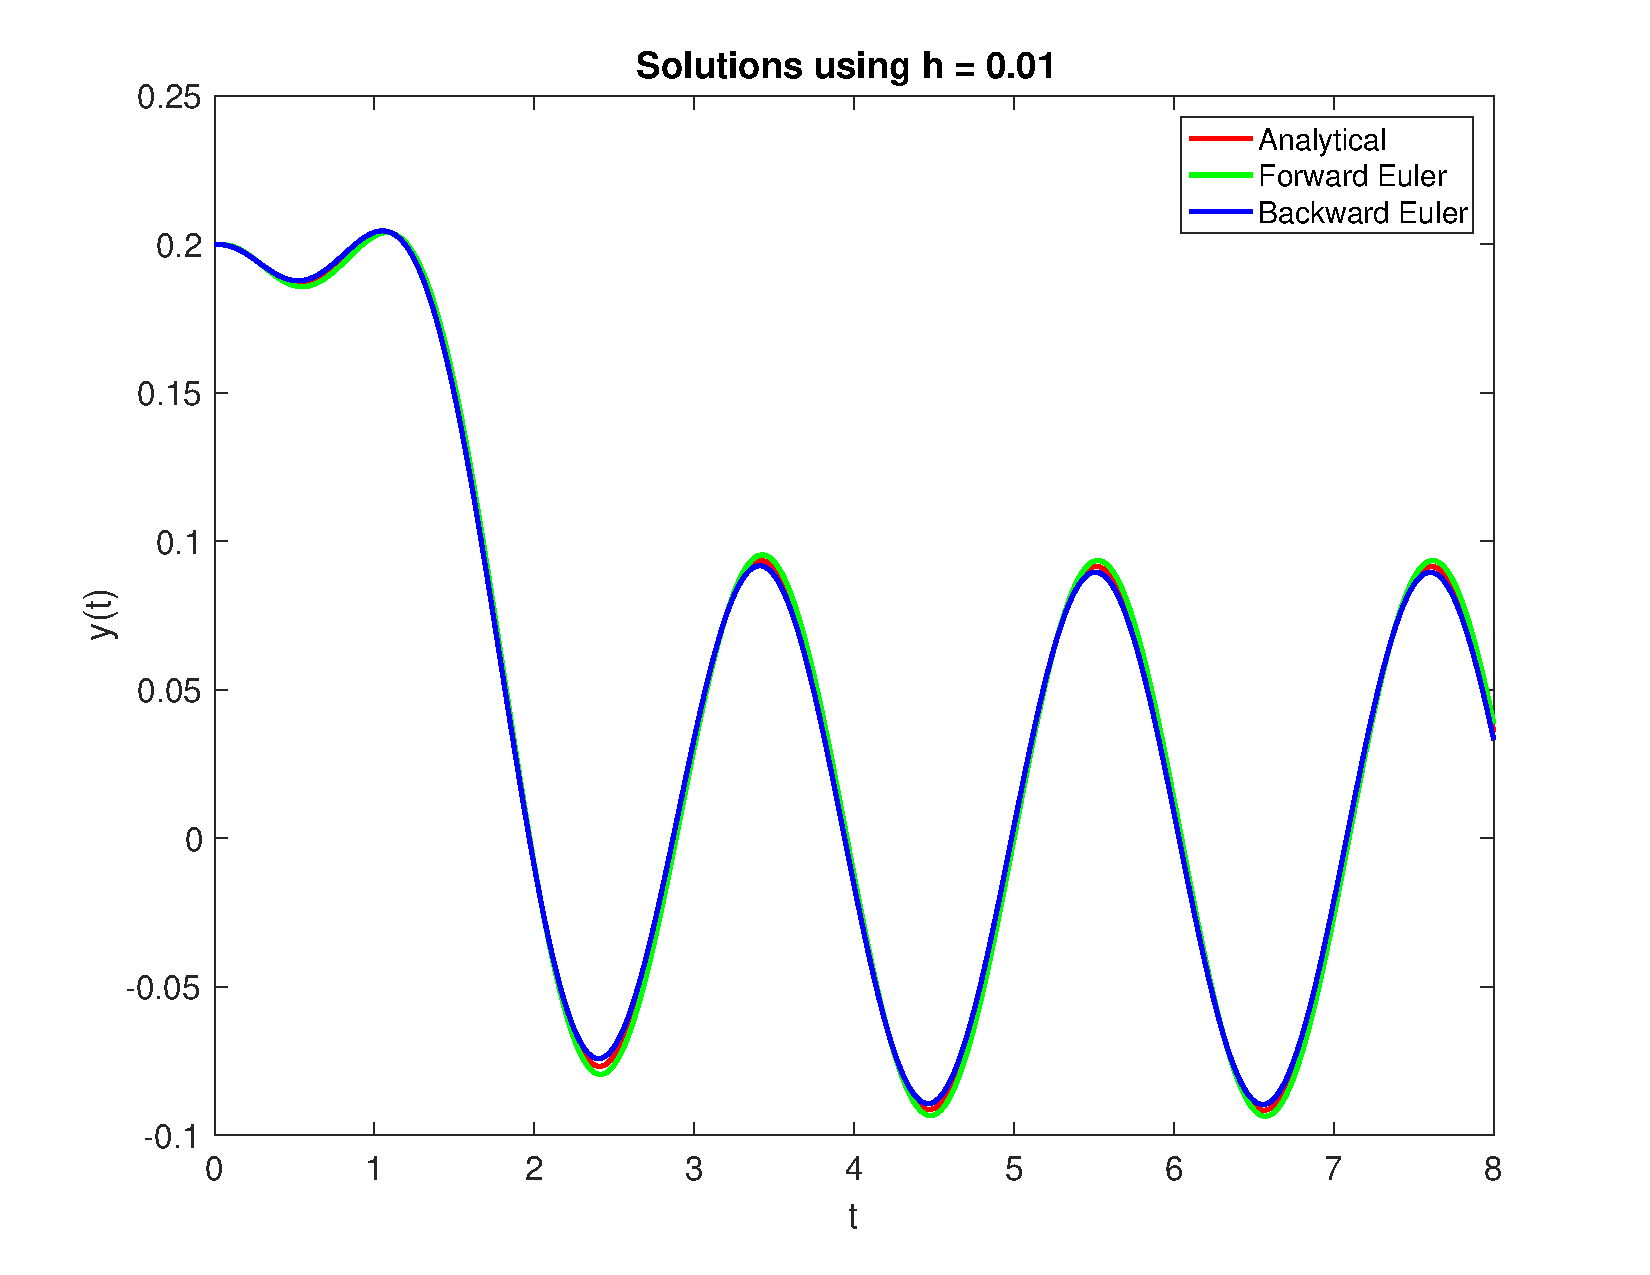
\includegraphics[width=\paperwidth]{h001.pdf}}
\noindent\makebox[\textwidth]{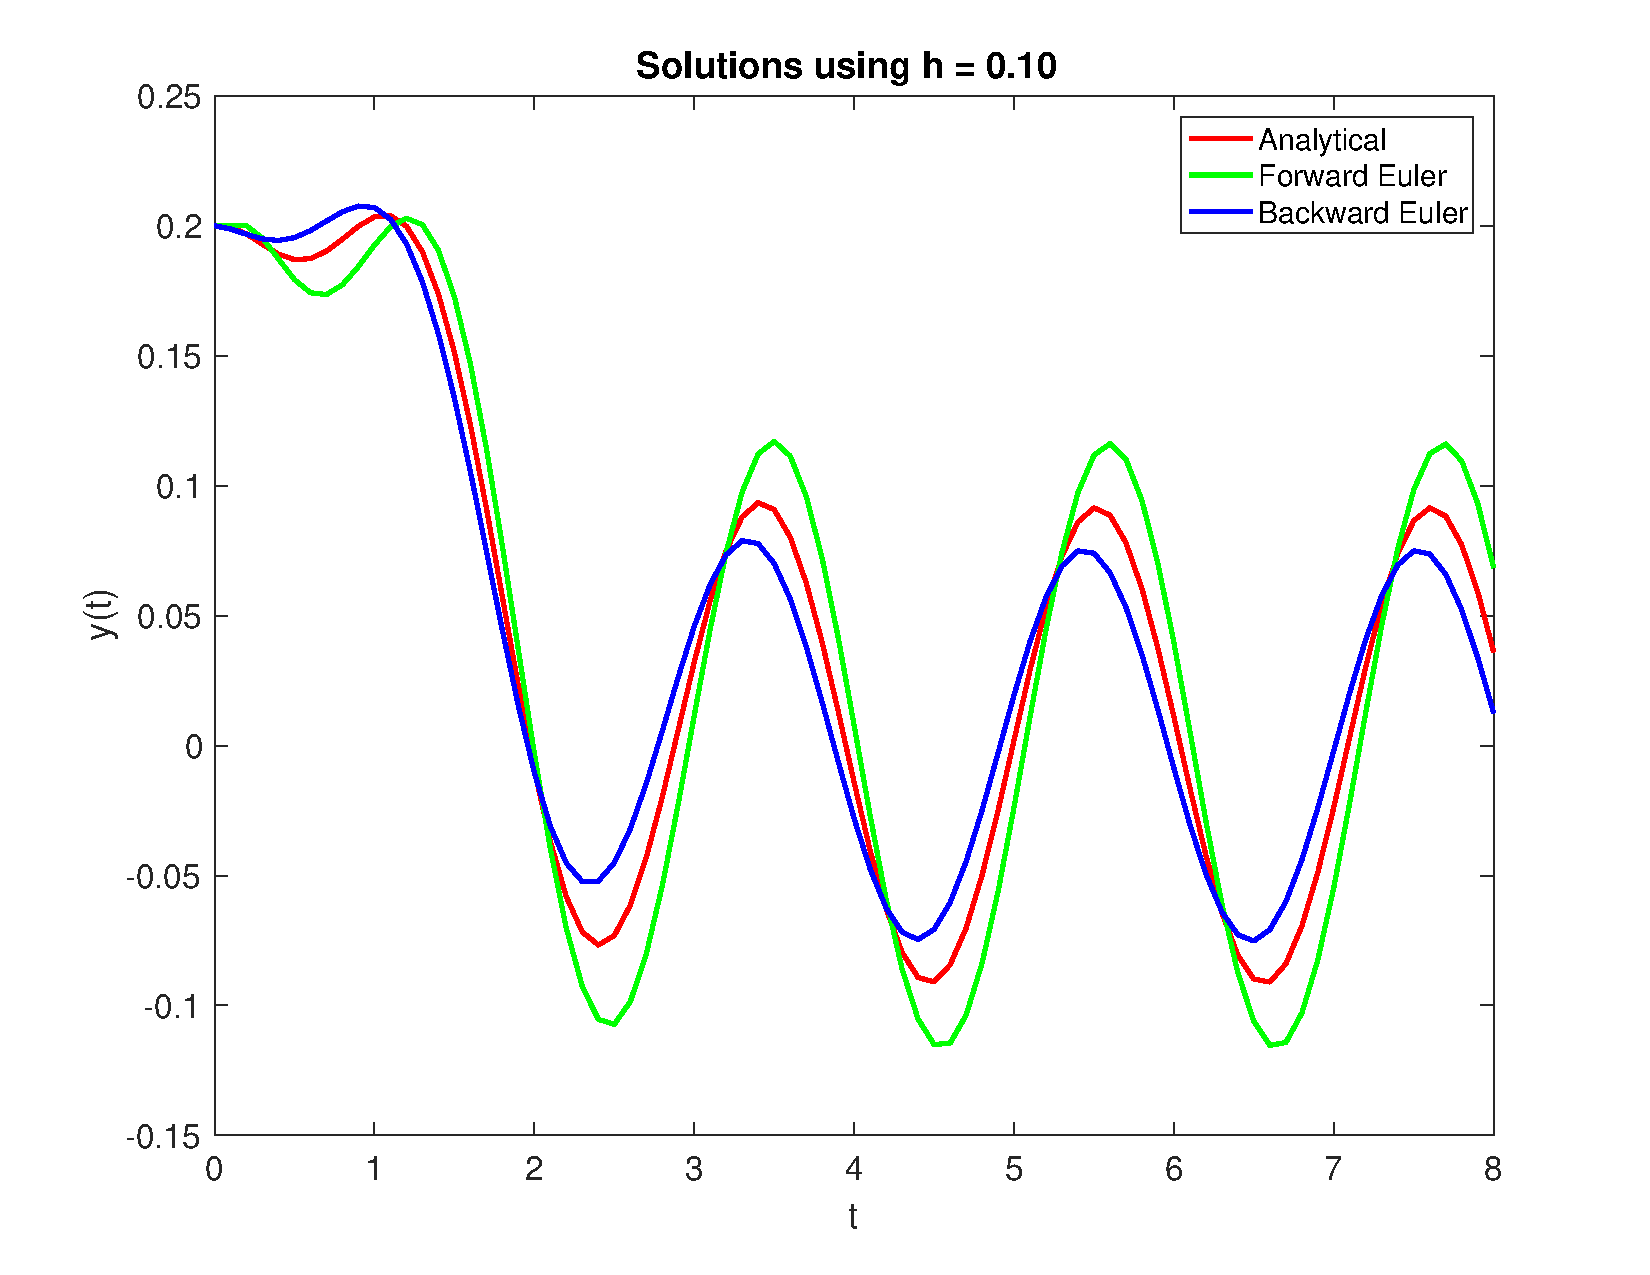
\includegraphics[width=\paperwidth]{h01.pdf}}
\end{document}